\chapter{Grundlagen}

Für die vorligendee Arbeit sind Kenntnisse in den Bereichen Laserlichtschneiden, Blechverarbeitung, Bildverarbeitung und Convolutional Neuroal Networks (CNNs) erforderlich. In diesem Kapitel werden die wichtigsten Grundlagen erläutert.

\section{Laserlichtschneiden}

Beim Laserlichtschneiden wird ein fokussierter Laserstrahl auf die Werkstückoberfläche gerichtet. Das Material schmilzt lokal auf und wird mit einem zugeführten Gas aus dem Schnittspalt ausgeblasen. So entsteht eine schmale, definierte Trennfuge. Die grundlegenden Begriffe und Kenngrößen (z.\,B.\ Strahlleistung, Strahlqualität, Fokuslage) sind in \parencite{ISO11145-2018} beschrieben.

In der Produktion kommen vor allem Faser- und Scheibenlaser zum Einsatz. CO\textsubscript{2}-Laser werden seltener verwendet. Faser- und Scheibenlaser erlauben hohe Energiedichten im Brennfleck und damit hohe Schnittgeschwindigkeiten, besonders bei dünnen bis mittleren Blechdicken. Die Wahl des Prozessgases beeinflusst Schnittqualität und Kantenfarbe. Beim Schneiden mit Stickstoff bildet sich kaum Oxid an der Schnittkante, die Kante bleibt hell und metallisch. Das ist vorteilhaft, weil in der Regel weniger Nacharbeit erforderlich ist, wie z.B dem Nachbürsten der Kante, so dass wieder eine metalische Oberfläche zu sehen ist. Beim Schneiden mit Sauerstoff reagiert das Material mit dem Gas und somit entsteht eine dunkle Oxidschicht, die die Kante verfärbt. Der Prozess kann zwar schneller sein, führt aber demanch zu zusätzlicher Nacharbeit, wenn eine helle und einwandfreie Kante gefordert ist.

Die wichtigsten Einstellgrößen dieser sind die Laserleistung, Schnittgeschwindigkeit, Fokuslage und Gasdruck. Eine höhere Leistung erlaubt höhere Geschwindigkeit, bis die Qualitätsgrenzen erreicht sind. Eine unpassende Fokuslage führt schnell zu Grat oder unvollständigem Materialaustrag. Der Gasdruck muss so gewählt werden, dass die Schmelze zuverlässig aus dem Schnittspalt entfernt wird, ohne die Kante aufzurauen. Für die Bewertung der Schnittqualität sind u.\,a.\ Grat und Rauheit relevant. ISO~9013 fasst hierfür Klassen und Toleranzen zusammen \parencite{ISO9013-2017}.

Für Edelstahl gelten gegenüber Baustahl angepasste Einstellungen. Gründe sind unter anderem eine höhere Reflexion und eine geringere Wärmeabfuhr. In der Praxis bedeutet das, dass die Leistung und die Fokuslage sorgfältig abgestimmt werden müssen. Die Geschwindigkeit muss demnach passend gewählt werden. Als Prozessgas wird meistens Stickstoff eingesetzt, um eine helle Kante und geringen Grat zu erreichen.

\section{Grat und Rauheit eines Blechteils}
\label{sec:grat-rauheit}

Für das Verständis der vorliegenden Arbeit sind Grat und Rauheit wichtige Kenngrößen der Schnittqualität. Dies wird in diesem Abschnitt erläutert.

Grat und Rauheit beschreiben die Qualität der Schnittkante. Der Grat ist ein aufgeworfener Materialrand an der Unterkante und entsteht durch unvollständigen Schmelzaustrag oder Anhaften von Schmelze im Schnittspalt. Die Rauheit beschreibt die feinen Höhenabweichungen der Schnittfläche entlang eines Profils \(Z(x)\).

Die in Tabelle~\ref{tab:symbole-rauheit-grat} zusammengefassten Formelzeichen werden in diesem Dokument verwendet.
\begin{table}[htbp]
  \centering
  \ra{1.2}
  \caption{Formelzeichen für Rauheit und Grat}
  \label{tab:symbole-rauheit-grat}
  \begin{tabular}{@{}lll@{}}
    \toprule
    Zeichen & Bedeutung & Einheit \\
    \midrule
    $Z(x)$      & gefiltertes Profil entlang der Auswertelänge $L$ & $\mu$m \\
    $Z_i$       & diskreter Profilwert an Position $x_i$            & $\mu$m \\
    $L$         & Auswertelänge                                      & mm \\
    $n$         & Anzahl der Stützstellen in $L$                     & -- \\
    $X_{s,j}$   & $j$-te Teilstrecke innerhalb von $L$               & mm \\
    $R_a$       & arithmetischer Mittenrauwert                       & $\mu$m \\
    $R_z$       & mittlere Rautiefe aus fünf Teilstrecken            & $\mu$m \\
    $P^{\max}_{j}$, $P^{\min}_{j}$ & höchster bzw.\ tiefster Punkt in $X_{s,j}$ & $\mu$m \\
    $h_b$       & Grathöhe an der unteren Schnittkante               & $\mu$m \\
    \bottomrule
  \end{tabular}
\end{table}

Die Berechnung der Kenngrößen folgt den nachfolgenden Rechenregeln. Der arithmetische Mittenrauwert \(R_a\) ist das Mittel der Beträge der Profilabweichung über die Auswertelänge \(L\) \parencite{MitutoyoQuickGuide}:
\[
R_a=\frac{1}{L}\int_{0}^{L}\lvert Z(x)\rvert\,\mathrm{d}x
\]
und in diskreter Form mit \(n\) Stützstellen \(Z_i\):
\[
R_a=\frac{1}{n}\sum_{i=1}^{n}\lvert Z_i\rvert.
\]
Die mittlere Rautiefe \(R_z\) wird über fünf Teilstrecken \(X_{s,1}\) bis \(X_{s,5}\) bestimmt \parencite{KeyenceISO4287}. In jeder Teilstrecke wird die Differenz zwischen höchstem und tiefstem Profilpunkt gebildet. \(R_z\) ist das arithmetische Mittel dieser fünf Differenzen:
\[
R_z=\frac{1}{5}\sum_{j=1}^{5}\bigl(P^{\max}_{j}-P^{\min}_{j}\bigr).
\]

Die Grathöhe \(h_b\) wird als maximale positive Auslenkung des Profils im Randbereich der unteren Schnittkante bestimmt. Grundlage ist dasselbe Profil \(Z(x)\) oder ein aus einer Punktwolke abgeleitetes Profil senkrecht zur Kante. Neben \(h_b\) können Breite und Form des Grates angegeben werden.
Die Profilwerte \(Z_i\) stammen aus einer 3D-Punktwolke oder aus einer bildbasierten Profilerfassung. Aus diesen Werten werden \(R_a\) und \(R_z\) berechnet. Die Grathöhe \(h_b\) wird im Kantenbereich aus demselben Profil ermittelt. Einen Überblick zum verwendeten 3D-Messsystem gibt Abschnitt~\ref{sec:3d-messsystem-keyence}.

Die Abbildung~\ref{fig:roughness-profile} zeigt das gefilterte Rauheitsprofil \(Z(x)\) über der Messstrecke \(X\).
Die rote Linie kennzeichnet \(R_a\), \(Z_i\) sind die diskreten Profilwerte und \(X_{s,j}\) die Teilstrecken für \(R_z\). Die Grathöhe \(h_b\) wird an der unteren Schnittkante als größte positive Auslenkung im Kantenfenster bestimmt.

\begin{figure}[htbp]
  \centering
  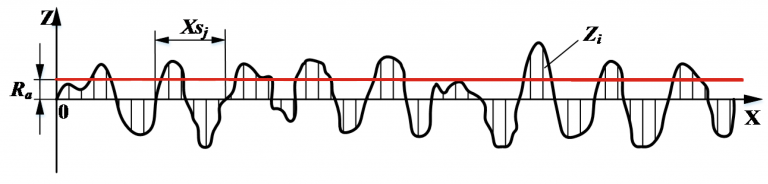
\includegraphics[width=\linewidth]{burr_roughness_schaubild.png}
  \caption[Schema zur Bestimmung der Rauheit]{Schema zur Bestimmung der Rauheit mit Profilwerten \(Z_i\), Teilstrecken \(X_{s,j}\) und markiertem \(R_a\) \parencite{Timesavers_Rauheit_Ra}.}
  \label{fig:roughness-profile}
\end{figure}

\section{Convolutional Neural Networks (CNNs)}
\label{sec:cnns}

Das vorliegende Kapitel soll ein Grundverständnis zu Convolutional Neural Networks (CNNs) vermitteln, da dies die Grundlage des Cutting Assistent ist, welcher in Kapitel~\ref{sec:cutting-assistent} beschrieben wird und als Bestandteil der Arbeit erweitert werden soll.

Convolutional Neural Networks (CNNs) sind neuronale Netze für Bilddaten. Sie bestehen aus wiederholten Blöcken aus Faltung (Convolution), nichtlinearer Aktivierung (z.\,B.\ ReLU) und Subsampling/Pooling sowie einem abschließenden Klassifikations- oder Regressionskopf aus vollverbundenen Schichten. Abbildung~\ref{fig:cnn-schema} zeigt dies am Beispiel eines Roboterbildes. Zu Beginn laufen kleine Filter (typisch $3{\times}3$) über das Pixelgitter und reagieren auf lokale Muster. In den ersten Schichten entstehen so Merkmalskarten für einfache Strukturen wie Kanten und Ecken, etwa an der Kontur des Kopfes oder entlang der Armsegmente des Roboters. Eine Aktivierungsfunktion unterdrückt schwache oder negative Antworten und erhöht den Kontrast zwischen relevanten und irrelevanten Bildbereichen. Pooling verdichtet die Merkmalskarten und macht die Darstellung unempfindlicher gegenüber kleinen Verschiebungen. Demnach ist die genaue Position der runden Augen oder Schrauben wird damit weniger wichtig als ihr Auftreten.

Mit zunehmender Tiefe kombinieren weitere Faltungen diese einfachen Muster zu komplexeren Teilen wie Gesicht, Gelenken oder ganzen Körpersegmenten. Am Ende wird die verdichtete Repräsentation \emph{geflattet} und von vollverbundenen Schichten zu einer Ausgabe verdichtet, etwa zu Klassenwahrscheinlichkeiten (\enquote{Roboter ja/nein}) oder zu kontinuierlichen Werten. Das Netzwerk lernt dabei sämtliche Filtergewichte gemeinsam, sodass frühe und späte Schichten aufeinander abgestimmt sind und eine konsistente Merkmals­hierarchie vom Lokalen zum Globalen entsteht \parencite{FischerPochwyt_NeuronaleNetze_2017}.

\begin{figure}[htbp]
  \centering
  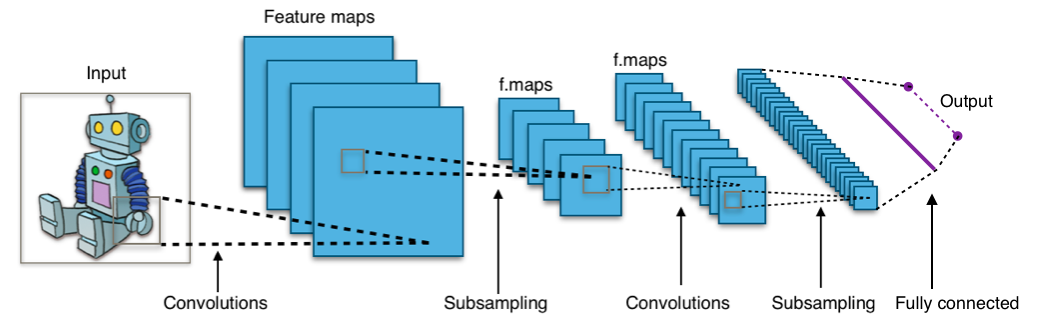
\includegraphics[width=0.9\linewidth]{CNNs.png}
  \caption[Schematischer Aufbau eines CNN]{Schematische Pipeline eines CNN am Beispiel eines Roboterbildes: Faltung extrahiert lokale Muster, Pooling verdichtet die Repräsentation, tiefere Stufen kombinieren Teile zu Objekten, die Entscheidung erfolgt in vollverbundenen Schichten \parencite{FischerPochwyt_NeuronaleNetze_2017}.}
  \label{fig:cnn-schema}
\end{figure}

Nach demselben Prinzip arbeitet der in dieser Arbeit weiterentwickelte \enquote{Cutting Assistent} (siehe Kapitel~\ref{sec:cutting-assistent}). Frühe Filter reagieren auf Kanten und Texturwechsel in Schnittkantenbildern, Pooling sorgt für Robustheit gegen kleine Lageänderungen, und tiefere Schichten fassen wiederkehrende Muster wie Riefen, Rauheitsstrukturen oder Gratbildung zusammen. Die abschließenden Schichten liefern je nach Aufgabe eine Klassifikation oder Regressionswerte wie Rauheit oder Grathöhe.
